\documentclass[12pt,a4paper]{article}

% ─── Packages ────────────────────────────────────────────────────────────────
\usepackage[french]{babel}
\usepackage[T1]{fontenc}
\usepackage[utf8]{inputenc}
\usepackage{color}
\usepackage{fancyhdr}
\usepackage{graphicx}
\usepackage{amsmath}
\usepackage{tcolorbox}
\usepackage{tabularx}
\usepackage{needspace}
\usepackage[justification=centering]{caption}
\usepackage{float}
\usepackage{hyperref}
\usepackage{cleveref}

\setlength{\headheight}{15pt}
\pagestyle{fancy}

\begin{document}

    \begin{figure}[t]
        \includegraphics[scale=0.5]{assets/logos/logo\_lmu.png}
        \hfill
        \includegraphics[scale=0.5]{assets/logos/logo\_ic2.png}
    \end{figure}

    \title{
        \textcolor{blue}{Le Mans Université}\\
        Licence Informatique \textit{2ème année}\\
        Module 174UP02 Rapport de Projet\\
        \textbf{Codenames}\\
        \vspace{0.5cm}
        \normalsize\url{https://github.com/noam120606/codenames-c}
    }
    \author{PIAU Romain - ROGER Noam \\QUINTON Chloé - MAUDET Mathis}
    \date{\today}
    \maketitle

    \newpage

    % ─── Table des matières ──────────────────────────────────────────────────────
    \tableofcontents

    \newpage 

    \section{Introduction}
    \label{sec:intro}
        Ce document présente le projet de jeu Codenames en C réalisé dans le cadre de
        la formation de L2 Informatique de l’Université Le Mans, sur la période de janvier à
        avril 2026. Ce projet a été développé en langage C et repose sur deux composantes
        principales : un client graphique utilisant la bibliothèque SDL2, et un serveur TCP
        gérant la logique de jeu et la communication réseau.\\
        Codenames est un jeu de société coopératif/compétitif dans lequel deux équipes
        s’affrontent pour identifier leurs mots-agents avant l’équipe adverse, en se basant sur des
        indices formulés par leur maître espion. Notre implémentation reprend fidèlement les règles
        officielles tout en y ajoutant plusieurs fonctionnalités originales décrites dans ce rapport.\\
        Le plan de ce rapport est le suivant : nous présenterons dans une première partie la
        conception du jeu (règles, scénarios d’utilisation et fonctionnalités), puis dans une deuxième
        partie l’organisation du travail en équipe. La troisième partie détaille les aspects techniques
        du développement (structures de données, algorithmes clés, interfaces graphiques et gestion
        du réseau). Nous montrerons ensuite l’architecture du code avant de conclure par un bilan
        du projet. Des annexes présentent les éléments additionnels permettant de compléter la
        compréhension du jeu et de son implémentation.

    \newpage
    \section{Conception}
    \label{sec:conception}

        \subsection{Présentation du jeu}

            \textit{Codenames} est un jeu d’association d’idées en équipes.
            Chaque équipe doit retrouver ses mots secrets à partir d’indices donnés par son espion.

            \begin{tcolorbox}[colback=blue!5,colframe=blue!50]
            \textbf{Objectif :} être la première équipe à retrouver tous ses mots.
            \end{tcolorbox}

            \begin{enumerate}

                \item Mise en place :

                    \begin{itemize}
                        \item Former 2 équipes : rouge et bleue
                        \item Choisir un espion par équipe
                        \item Disposer 25 mots en grille (5x5)
                        \item Tirer une carte clé au hasard\\ \textbf{Important :} La carte clé indique :
                        \begin{itemize}
                            \item 9 mots pour une équipe (celle qui commence)
                            \item 8 mots pour l’autre
                            \item 7 civils
                            \item 1 assassin
                        \end{itemize}
                    \end{itemize}

                \vspace{0.5cm}
                \item Déroulement d’un tour

                    \begin{enumerate}
                        \item Donner un indice

                            L'espion doit dire :

                            \begin{itemize}
                                \item Un mot unique
                                \item Un nombre
                            \end{itemize}

                            \vspace{0.5cm}

                            \needspace{5\baselineskip}

                            \textbf{Exemple :}

                            \begin{tcolorbox}
                            Indice : \textbf{Animal 2}
                            \end{tcolorbox}

                            Cela signifie que 2 mots sur la table sont liés à "animal".

                            \vspace{0.5cm}
                            
                            \textbf{Règles strictes pour les indices}

                            \begin{itemize}
                                \item Un seul mot (pas de phrase)
                                \item Pas un mot présent sur la table
                                \item Pas une partie d’un mot (ex : "auto" pour "automobile" interdit)
                                \item Pas de traduction directe (ex : dire "dog" pour "chien")
                                \item Pas de communication non verbale
                            \end{itemize}

                        \vspace{0.5cm}
                        
                        \item Phase de devinettes

                            Les joueurs peuvent proposer des mots.

                            \begin{itemize}
                                \item Nombre minimum de propositions = nombre annoncé
                                \item Nombre maximum de propositions = nombre annoncé + 1
                            \end{itemize}

                            \vspace{0.5cm}

                            \textbf{Exemple :}

                            \begin{tcolorbox}
                            Indice : \textbf{Animal 2}
                            \end{tcolorbox}

                            → L’équipe doit proposer au minimum 2 mots mais peu en proposer jusqu’à 3.

                            \vspace{0.5cm}

                            Résultat des choix

                            \begin{enumerate}

                                \item \textbf{Bon mot}

                                    \begin{itemize}
                                        \item On recouvre avec la couleur de l’équipe
                                        \item L’équipe peut continuer
                                    \end{itemize}

                                \item \textbf{Mot neutre}

                                    \begin{itemize}
                                        \item Tour terminé immédiatement
                                    \end{itemize}

                                \item \textbf{Mot adverse}

                                    \begin{itemize}
                                        \item Tour terminé
                                        \item Aide l’équipe adverse
                                    \end{itemize}

                                \item \textbf{Assassin}

                                    \begin{itemize}
                                        \item \textcolor{red}{Effet : défaite immédiate}
                                    \end{itemize}

                            \end{enumerate}

                    \end{enumerate}
                
                \vspace{0.5cm}
                \needspace{3\baselineskip}
                \item Fin de partie

                    \begin{itemize}
                        \item Une équipe gagne si elle trouve tous ses mots
                        \item Une équipe perd immédiatement si elle choisit l’assassin
                    \end{itemize}
                
                \vspace{0.5cm}
                \Needspace{5\baselineskip}
                \item Règles avancées

                    Indice avec 0

                    \begin{tcolorbox}
                    Exemple : \textbf{Animal 0}
                    \end{tcolorbox}

                    Signifie :
                    Aucun mot restant n’est lié à "animal".

                    → Permet d’éviter certains pièges.

            \end{enumerate}
        
        \Needspace{10\baselineskip}
        \subsection{Notre adaptation numérique}
            Notre version numérique de Codenames vise à recréer l'expérience du jeu de société tout en offrant des fonctionnalités supplémentaires pour améliorer l'interaction et la convivialité.

            \vspace{0.5cm}

            Fonctionnalités principales :
            \begin{enumerate}
                \item Interface utilisateur intuitive grâce à SDL
                    \begin{itemize}
                        \item différentes interfaces créées pour chaque étape (menu, lobby, jeu),
                        \item gestion avancée de boutons et inputs,
                        \item bandeau d'informations (affichage ping et fps, réglage du volume et de la luminosité, règles du jeu).
                    \end{itemize}
                \item Gestion automatique des règles du jeu, le code permet  
                    \begin{itemize}
                        \item de vérifier la validité des indices donnés par les espions,
                        \item de gérer les différentes phases du jeu (donner un indice, devinettes, fin de partie),
                        \item d'appliquer les conséquences des choix des joueurs (bon mot, mot neutre, mot adverse, assassin).
                    \end{itemize}
                \item Possibilité de jouer en ligne avec des amis grâce à la création de lobbies privés
                \item Système de chat intégré pour communiquer entre les joueurs
                \item Historique des indices 
            \end{enumerate}

    \newpage
    \section{Organisation du travail}
    \label{sec:organisation}
        \renewcommand{\arraystretch}{1.3}
        \setlength{\tabcolsep}{8pt}
        \begin{table}[h]
        \centering
        \begin{tabularx}{\textwidth}{|>{\raggedright\arraybackslash}X|c|c|c|c|}
        \hline
        \textbf{Tâches} & \textbf{Noam} & \textbf{Romain} & \textbf{Chloé} & \textbf{Mathis} \\
        \hline
        Conception de la structure du code & 40\% & 30\% & 15\% & 15\% \\
        \hline
        Fonctions principales (serveur) & 30\% & 30\% & 20\% & 20\% \\
        \hline
        Fonctions principales (client) & 20\% & 20\% & 30\% & 30\% \\
        \hline
        Gestion des différentes scènes de l'interface graphique & 10\% & 30\% & 30\% & 30\% \\
        \hline
        Gestion du lobby & 20\% & 20\% & 15\% & 45\% \\
        \hline
        Gestion des fonctions du jeu & 25\% & 25\% & 25\% & 25\% \\
        \hline
        Rédaction du rapport de projet & 15\% & 15\% & 55\% & 15\% \\
        \hline
        Tests et débogage & 25\% & 25\% & 25\% & 25\% \\
        \hline
        \end{tabularx}
        \caption{Répartition des tâches entre les membres de l'équipe}
        \end{table}

    \newpage
    \section{Développement}
    \label{sec:developpement}

        \subsection{Structure du code}

        Le code du jeu est structuré de la manière suivante :

        \begin{itemize}
            \item Deux parties principales : client et serveur
            \item Un dossier de tests
            \item Un dossier de documentation
            \item Un dossier rapport 
            \item Un fichier README.md pour expliquer les principales fonctionnalités du jeu et les instructions d'installation et d'utilisation
            \item Un fichier TODO.md pour suivre les tâches à accomplir et les fonctionnalités à implémenter
            \item Un fichier .gitignore pour exclure les fichiers temporaires et les ressources non nécessaires du dépôt Git
            \item Un fichier LICENSE pour spécifier les conditions de distribution et d'utilisation du code
            \item Un fichier setup pour faciliter l'installation des dépendances et la configuration de l'environnement de développement
            \item Un fichier Doxyfile pour la génération de la documentation avec Doxygen
        \end{itemize}

        \vspace{0.5cm}

        Les parties client et serveur sont les plus développées et contiennent les fonctionnalités principales du jeu. 
        Elles partagent une structure similaire pour faciliter la maintenance et la compréhension du code.

        \vspace{0.5cm}

        \begin{enumerate}
            \item \textbf{Points communs des deux parties}
                \begin{itemize}
                    \item Dossier assets : contient les ressources graphiques, textuelles ou sonores du jeu
                    \item Dossier lib : contient les fichiers d’en-tête et les bibliothèques
                    \item Dossier src : contient le code source
                    \item Fichier Makefile : pour la compilation du projet
                    \item Fichier run : pour lancer le jeu
                \end{itemize}
            \item \textbf{Côté client}
                \begin{itemize}
                    \item Bibliothèques SDL compilés (ajouté par le script setup)
                    \item Gestion de l'interface graphique (menu, lobby, jeu) 
                    \item Traitement des boutons, inputs utilisateur, crossfader, bandeau d'informations...
                    \item Communication avec le serveur (envoi des actions du joueur, réception des mises à jour du jeu)
                \end{itemize}
            \item \textbf{Côté serveur}
                \begin{itemize}
                    \item Gestion des connexions clients
                    \item Implémentation de la logique du jeu
                \end{itemize}
        \end{enumerate}

        \subsection{Principales structures de données}

        \begin{itemize}
            \item \textbf{AppContext} : contient les informations sur l’état de l’application.\\
                Utilité : centraliser les données et les ressources du jeu pour faciliter la gestion de l’état et de l’affichage.\\
                Détails :
                \begin{itemize}
                    \Needspace{4\baselineskip}
                    \item \textbf{Gérer l’affichage SDL}
                    \begin{itemize}
                        \item \texttt{window} $\rightarrow$ la fenêtre du jeu
                        \item \texttt{renderer} $\rightarrow$ le moteur de rendu graphique
                        \item \texttt{bg\_color} $\rightarrow$ couleur de fond
                    \end{itemize}

                    \Needspace{3\baselineskip}
                    \item \textbf{Gérer l’état du jeu}
                    \begin{itemize}
                        \item \texttt{app\_state} $\rightarrow$ menu, lobby, en partie, etc.
                        \item \texttt{lobby} $\rightarrow$ données du lobby (joueurs, salle, etc.)
                    \end{itemize}

                    \Needspace{5\baselineskip}
                    \item \textbf{Gérer le joueur}
                    \begin{itemize}
                        \item \texttt{player\_role} $\rightarrow$ agent ou espion
                        \item \texttt{player\_team} $\rightarrow$ équipe
                        \item \texttt{player\_id} $\rightarrow$ identifiant serveur
                        \item \texttt{player\_uuid}, \texttt{player\_name} $\rightarrow$ identité persistante
                    \end{itemize}

                    \Needspace{3\baselineskip}
                    \item \textbf{Gérer la connexion réseau}
                    \begin{itemize}
                        \item \texttt{sock} $\rightarrow$ identifiant réseau
                        \item \texttt{ping\_ms} $\rightarrow$ latence avec le serveur
                    \end{itemize}

                    \Needspace{5\baselineskip}
                    \item \textbf{Gérer le timing et les performances}
                    \begin{itemize}
                        \item \texttt{clock} $\rightarrow$ nombre de frames écoulées
                        \item \texttt{fps} $\rightarrow$ images par seconde
                        \item \texttt{frame\_start\_time} $\rightarrow$ début de la frame en cours
                        \item \texttt{last\_fullscreen\_toggle\_ms} $\rightarrow$ évite les toggles rapides
                    \end{itemize}

                    \Needspace{3\baselineskip}
                    \item \textbf{Gérer l’audio}
                    \begin{itemize}
                        \item \texttt{music\_volume} $\rightarrow$ volume de la musique
                        \item \texttt{sound\_effects\_volume} $\rightarrow$ volume des effets sonores
                    \end{itemize}

                    \Needspace{2\baselineskip}
                    \item \textbf{Gérer la luminosité} 
                    \begin{itemize}
                        \item \texttt{global\_luminosity} $\rightarrow$ luminosité globale 
                    \end{itemize}

                    \Needspace{3\baselineskip}
                    \item \textbf{Gérer la fenêtre}
                    \begin{itemize}
                        \item taille et position en mode fenêtré \\
                            (\texttt{windowed\_width}, \texttt{windowed\_height}, etc.)
                    \end{itemize}

                    \Needspace{2\baselineskip}
                    \item \textbf{Informations générales}
                    \begin{itemize}
                        \item \texttt{version} $\rightarrow$ version du jeu
                    \end{itemize}
                \end{itemize}
        \end{itemize}

        \vspace{0.5cm}

        \needspace{6\baselineskip}
        \begin{itemize}
            \item \textbf{Codenames} : Structure principale du serveur de Codenames.\\
                Utilité : regrouper tous les composants essentiels du serveur en un seul endroit.\\
                Détails :
                \begin{itemize}
                    \item \texttt{tcp} $\rightarrow$ gestionnaire du serveur TCP (sockets, clients, etc.)
                    \item \texttt{lobby} $\rightarrow$ gestionnaire des lobbies (parties en attente, joueurs, etc.)
                    \item \texttt{version} $\rightarrow$ version du serveur
                \end{itemize}
        \end{itemize}

        \subsection{Interface graphique}

        Codenames utilise la bibliothèque SDL pour créer une interface graphique immersive et interactive.
        L'interface est conçue pour être intuitive et facile à naviguer, avec des éléments visuels clairs et des animations fluides.
        Pour cela, nous avons développé plusieurs composants graphiques, tels que des boutons, des inputs, des crossfaders, etc.
        De plus, les différentes étapes du jeu (menu, lobby, partie) ont chacune leur propre interface adaptée à leurs fonctionnalités spécifiques.

        \needspace{10\baselineskip}

        \begin{figure}[H]
            \centering
            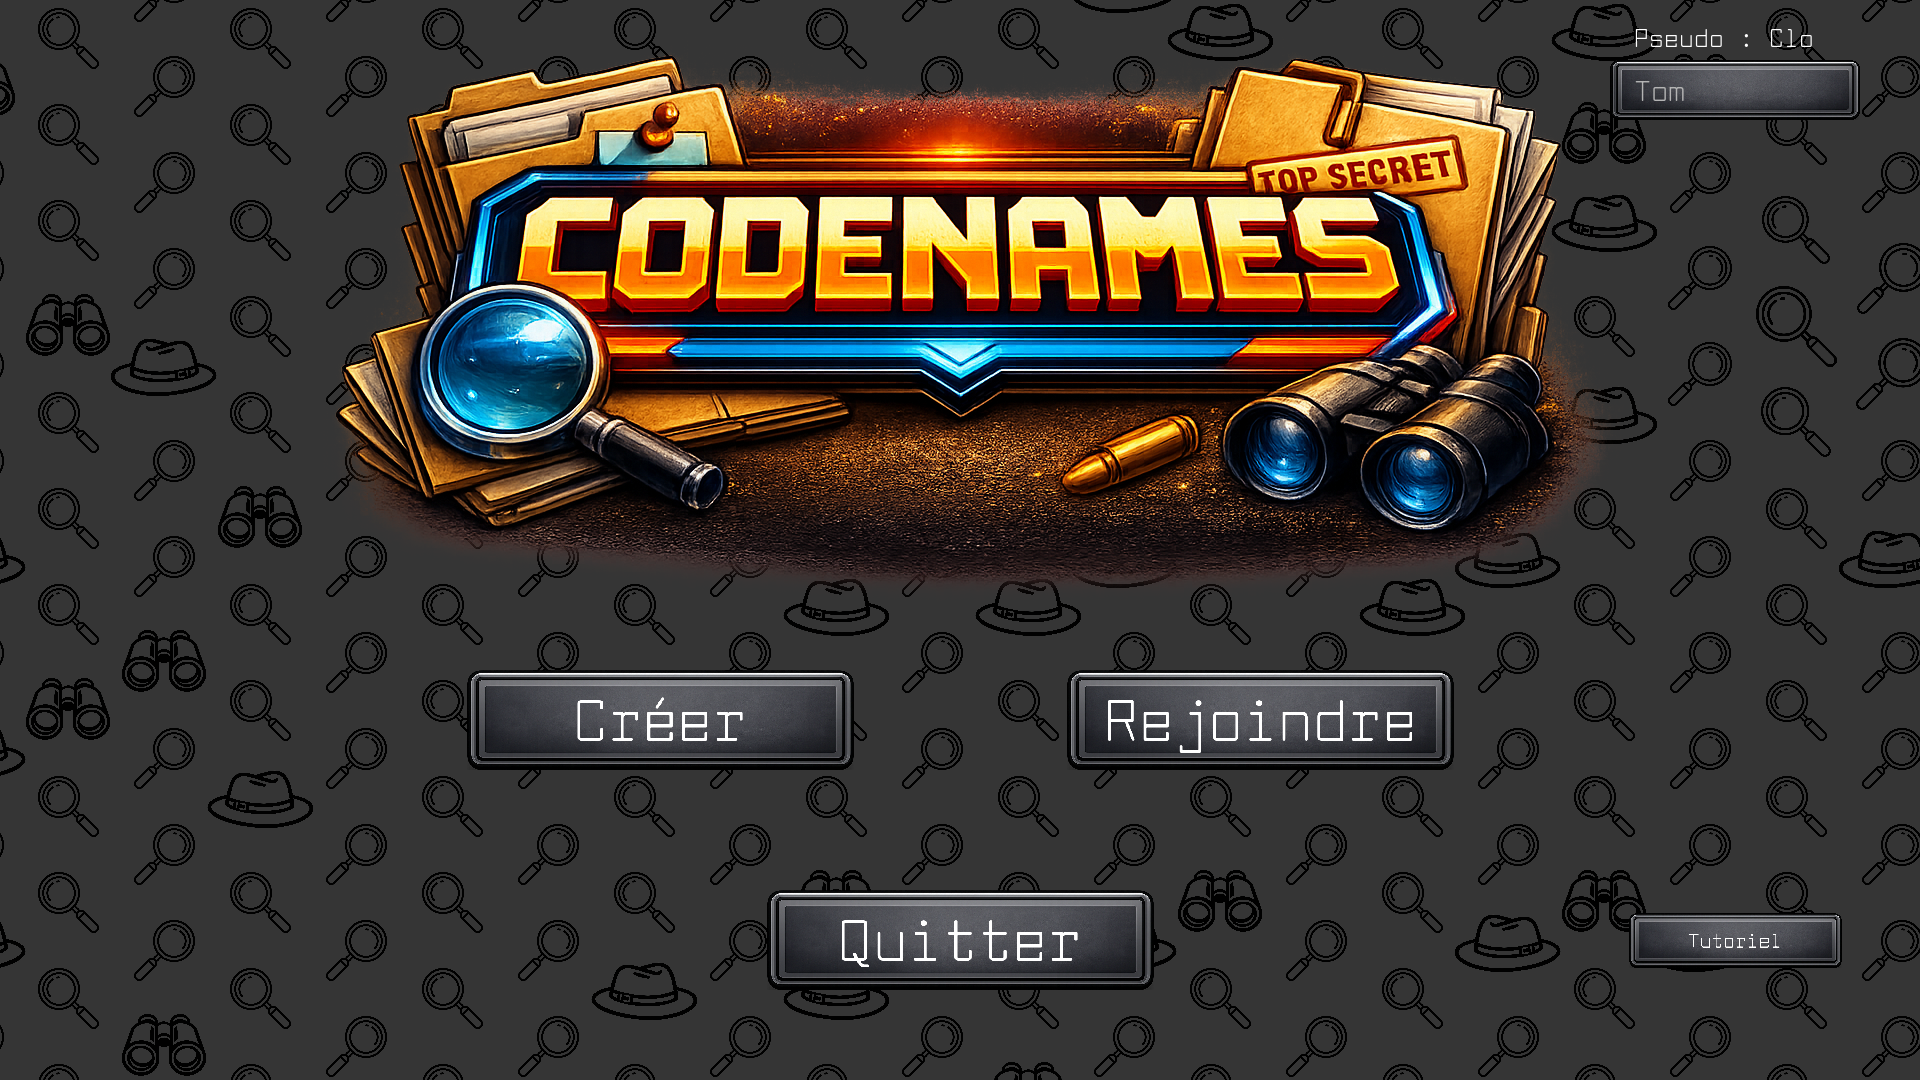
\includegraphics[width=\textwidth]{assets/interface_graphique/menu.png}
            \caption{Interface du menu principal}
            \label{fig:menu}
        \end{figure}

        \needspace{7\baselineskip}
        Dans la figure \ref{fig:menu}, on peut voir l'interface du menu principal, qui permet aux joueurs de 
        \begin{itemize}
            \item choisir leur pseudo grâce à l'input en haut à droite,
            \item créer un lobby avec le bouton \og Créer \fg{},
            \item rejoindre un lobby avec le bouton \og Rejoindre \fg{},
            \item accéder au tutoriel avec le bouton \og Tutoriel \fg{},
            \item quitter le jeu avec le bouton \og Quitter \fg{}.
        \end{itemize}
        
        \begin{figure}[H]
            \centering
            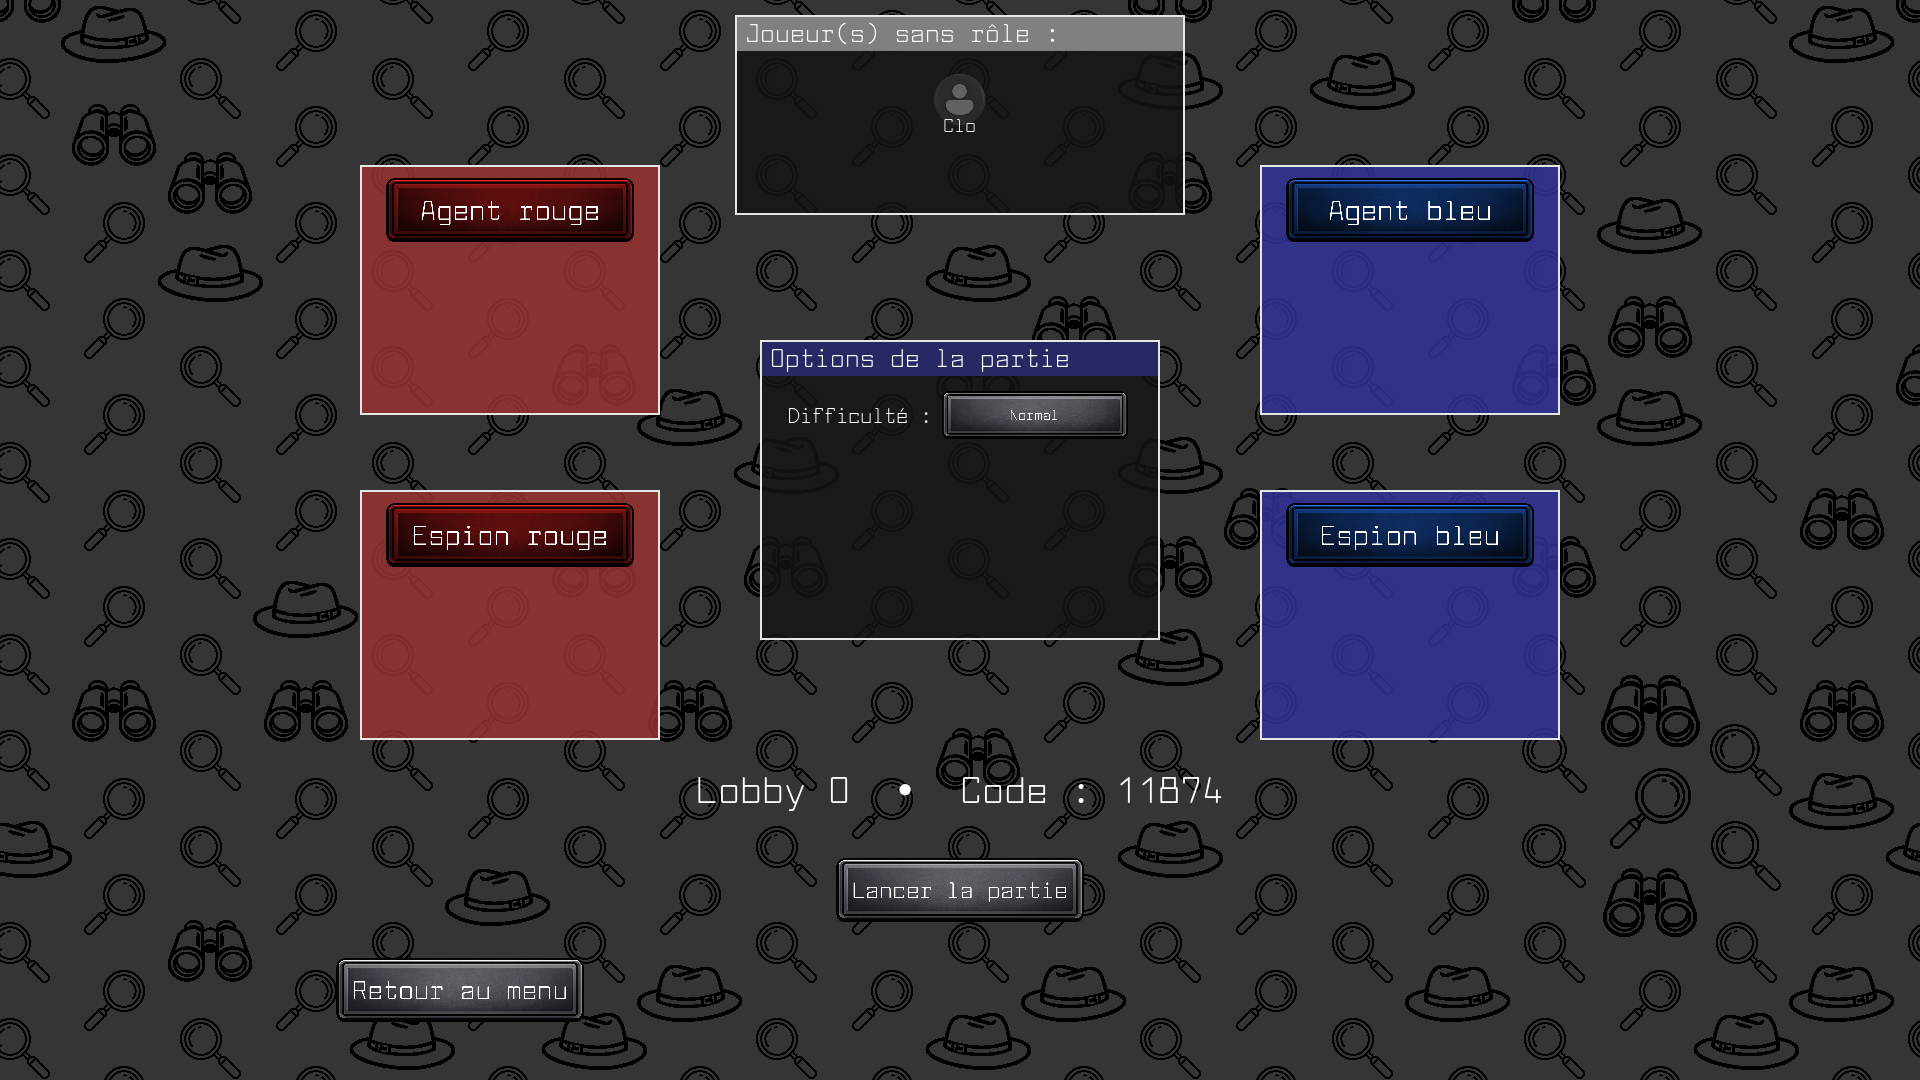
\includegraphics[width=\textwidth]{assets/interface_graphique/lobby.png}
            \caption{Interface du lobby}
            \label{fig:lobby}
        \end{figure}

        La figure \ref{fig:lobby} montre l'interface du lobby, où les joueurs peuvent 
        \begin{itemize} 
            \item voir les autres participants représentés par un icône de joueur et leur pseudo, 
            \item choisir leur équipe et leur rôle en cliquant sur les boutons correspondants,
            \item choisir la difficulté en cliquant sur les boutons correspondants (uniquement faisable par le créateur du lobby),
            \item attendre le début de la partie, lancé par le créateur du lobby avec le bouton \og Lancer la partie \fg{}. 
        \end{itemize}

        \begin{figure}[H]
            \centering
            \includegraphics[width=\textwidth]{assets/interface_graphique/jeu\_espion.png}
            \caption{Interface du jeu pour un espion}
            \label{fig:jeu_espion}
        \end{figure}

        \begin{figure}[H]
            \centering
            \includegraphics[width=\textwidth]{assets/interface_graphique/jeu\_agent.png}
            \caption{Interface du jeu pour un agent}
            \label{fig:jeu_agent}
        \end{figure}

        \needspace{5\baselineskip}
        Dans les figures \ref{fig:jeu_espion} et \ref{fig:jeu_agent}, on peut voir les interfaces du jeu pour un espion et un agent, sur chacune, on retrouve
        \begin{itemize}
            \item la grille de mots, avec les mots affichés dans la couleur correspondante pour les espions, et affichés de couleur neutres pour les agents,
            \item un chat en haut à droite pour communiquer entre les joueurs,
            \item deux historiques des indices en bas pour suivre les indices donnés par les espions (à gauche pour l'équipe rouge, à droite pour l'équipe bleue),
            \item un input pour que les agents puissent proposer leur indice, suivi d'un input pour choisir le nombre de mots correspondants à l'indice et enfin un bouton de validation pour envoyer leur proposition.
        \end{itemize}


        \needspace{10\baselineskip}
        \subsection{Gestion des parties}

        La gestion des parties est assurée par le serveur, qui maintient l'état de chaque partie en cours et gère les interactions entre les joueurs.
        Le serveur organise les différentes composantes du jeu de manière structurée, telles que les joueurs, les lobbies, les cartes, etc.
        Lorsqu'un joueur rejoint un lobby, le serveur met à jour l'état du lobby et informe les autres joueurs du nouvel arrivant.
        Lorsque la partie commence, le serveur gère les différentes phases du jeu (donner un indice, choisir un mot, fin de partie) en appliquant les règles du jeu et en envoyant les mises à jour aux clients.
        Le client est lui responsable de la validation des indices donnés par les espions, en vérifiant qu'ils respectent les règles du jeu (un seul mot, pas de mot présent sur la table, etc.) avant de les accepter et de les transmettre aux clients.

        \vspace{0.5cm}

        Au début de la partie, le serveur attribue les rôles d'espion et d'agent aux joueurs en fonction de leurs choix dans le lobby.
        Le serveur choisit ensuite les mots de la partie en sélectionnant aléatoirement 25 mots parmi une liste prédéfinie selon le choix de difficulté défini dans le lobby.
        Il attribue ensuite des couleurs à chaque mot en veillant à ce que les règles du jeu soient respectées (9 mots pour l'équipe qui commence, 8 pour l'autre, 7 civils et 1 assassin).
        Il est toutefois possible de modifier le nombre d'assassins dans le lobby (1, 2 ou 3).
        Puis les cartes sont mélangées pour créer la grille de mots finale.

        \vspace{0.5cm}

        Durant la partie, les équipes joueront à tour de rôle, les premiers à jouer auront donc un mot de plus à révéler que les autres.
        Les espions sont toujours les premiers à jouer, ils choisissent un mot et un nombre pour donner un indice à leur équipe, la validité de l'indice est vérifiée avant d'être transmise aux agents.
        Ensuite, ces agents peuvent proposer des mots en fonction de l'indice donné.
        Une fois validé, chaque mot est envoyé au serveur qui applique les conséquences de chaque choix.
        \begin{itemize}
            \item Si le mot appartient à l'équipe, il est recouvert par la bonne couleur et les agents peuvent continuer à jouer.
            \item Si le mot est neutre, il est recouvert par une couleur neutre et le tour de l'équipe est stoppé.
            \item Si le mot appartient à l'équipe adverse, il est recouvert de leur couleur et le tour de l'équipe est stoppé.
            \item Si le mot est l'assassin, l'équipe perd immédiatement la partie.
        \end{itemize}
        La partie continue jusqu'à ce qu'une équipe trouve tous ses mots ou que l'assassin soit révélé, entraînant la défaite immédiate de l'équipe concernée.

    \newpage
    \section{Bilan et conclusion}
        \label{sec:bilan}

        Les objectifs initiaux du projet ont été atteints et une version numérique du jeu de société Codenames a pu être réalisée avec une interface graphique immersive et des fonctionnalités complètes.
        Des fonctionnalités supplémentaires ont également pu être intégrées, telles que le chat en ligne, l'historique des indices, le tutoriel, le bandeau d'informations, etc.
        Les objectifs, choix de structure du code, de l'interface graphique et de la gestion des parties n'ont cessé de changer lors de la conception et de la mise en œuvre du projet, notamment suite à la rencontre de problemes techniques ou de changements d'avis des membres de l'équipe.
        Cependant, grâce à une bonne communication et une répartition efficace des tâches, les difficultés ont pu être surmontées et un projet fonctionnel et satisfaisant a pu être accompli.

    \newpage
    \section{Annexes}

    \subsection{Bandeau d'informations}
    Le bandeau d'informations est un élément de l'interface graphique qui permet d'afficher des informations utiles aux joueurs pendant la partie, ainsi que de régler certains paramètres du jeu.
    Il sort de la gauche de l'écran  lorsque la souris y est placée et contient
    \begin{itemize}
        \item l'affichage du ping serveur et des performances du jeu (FPS),
        \item les crossfaders pour régler la luminosité, le volume de la musique et des effets sonores,
        \item les règles du jeu.
    \end{itemize}

    \begin{figure}[H]
        \centering
        \includegraphics[width=\textwidth]{assets/annexes/bandeau/bandeau.png}
        \caption{Bandeau d'informations}
        \label{fig:bandeau}
    \end{figure}

    \newpage
    \subsection{Tutoriel}
    Un tutoriel a été intégré au menu principal pour permettre aux joueurs de découvrir l'interface du jeu et les fonctionnalités de notre version numérique.
    \begin{figure}[H]
        \centering
        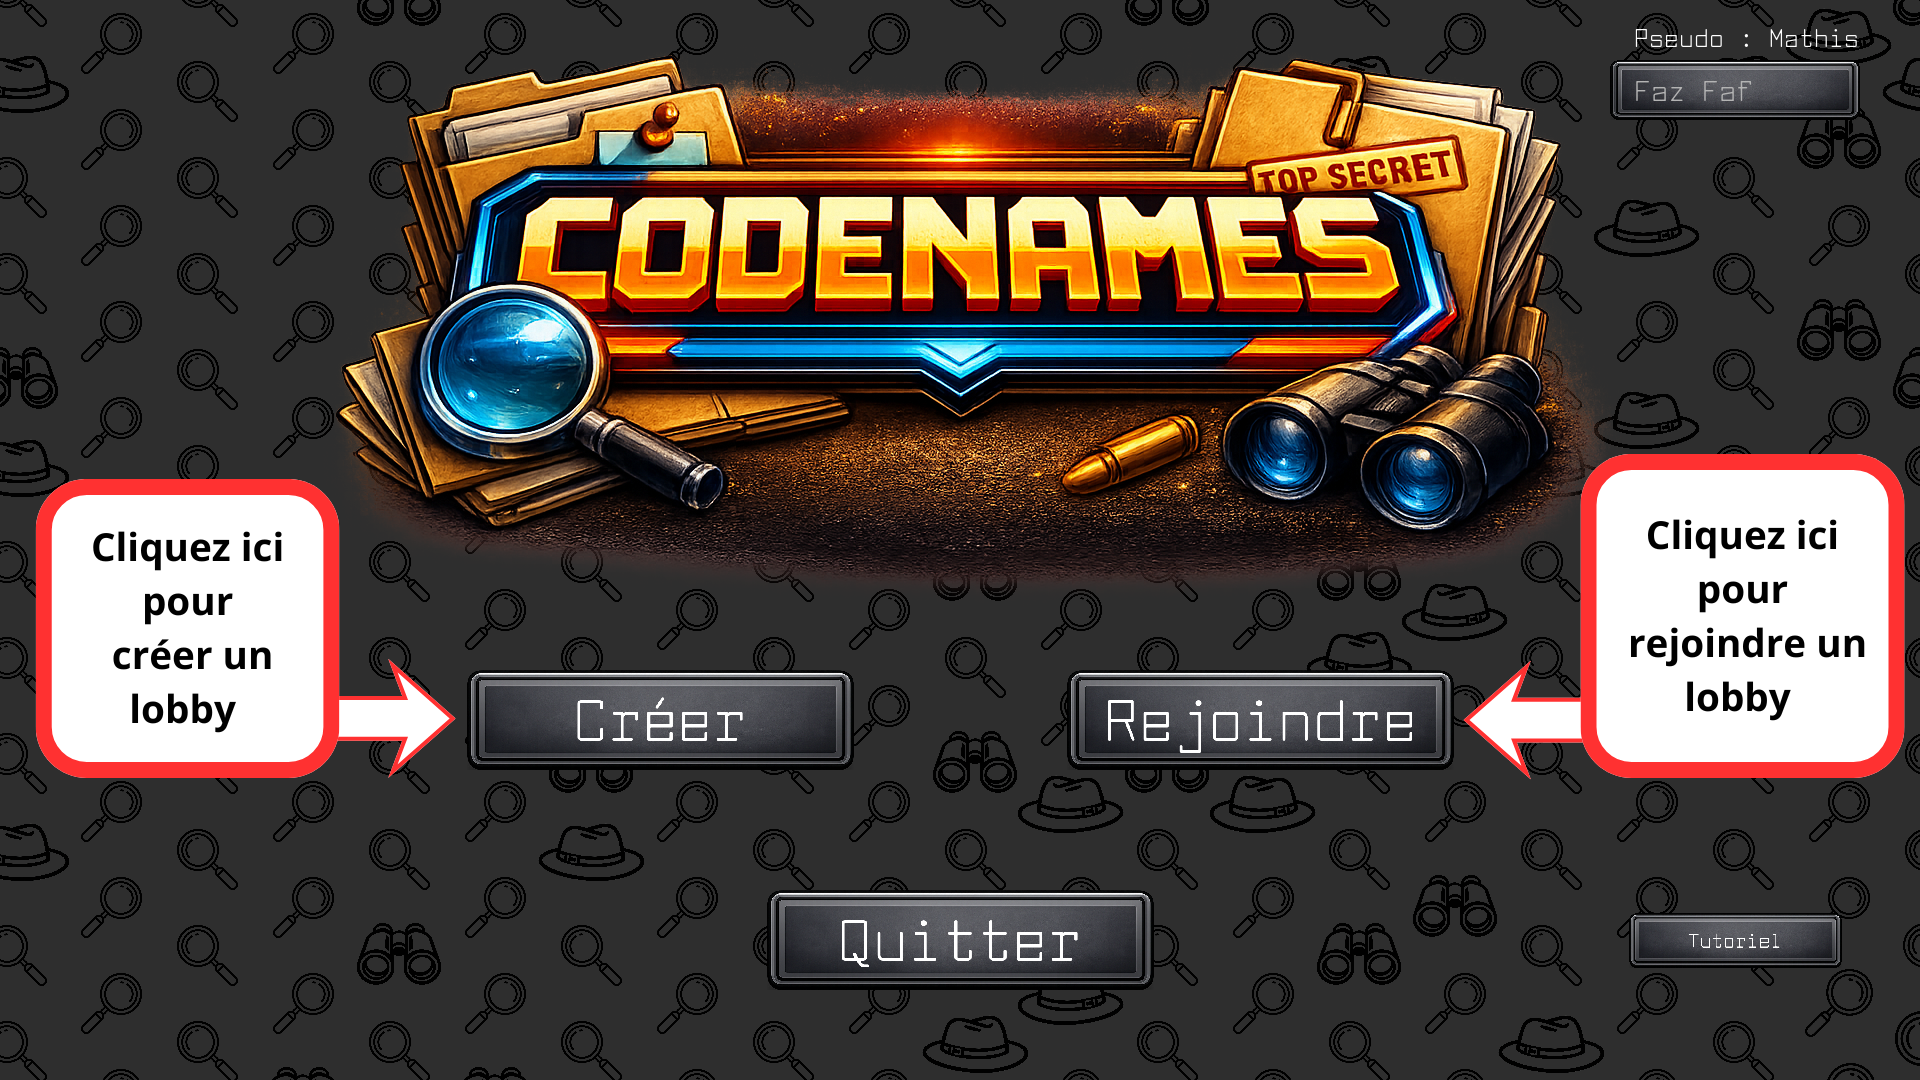
\includegraphics[width=\textwidth]{assets/annexes/tuto/tuto1.png}
        \caption{Page 1 du tutoriel}
        \label{fig:tuto1}
    \end{figure}
    \begin{figure}[H]
        \centering
        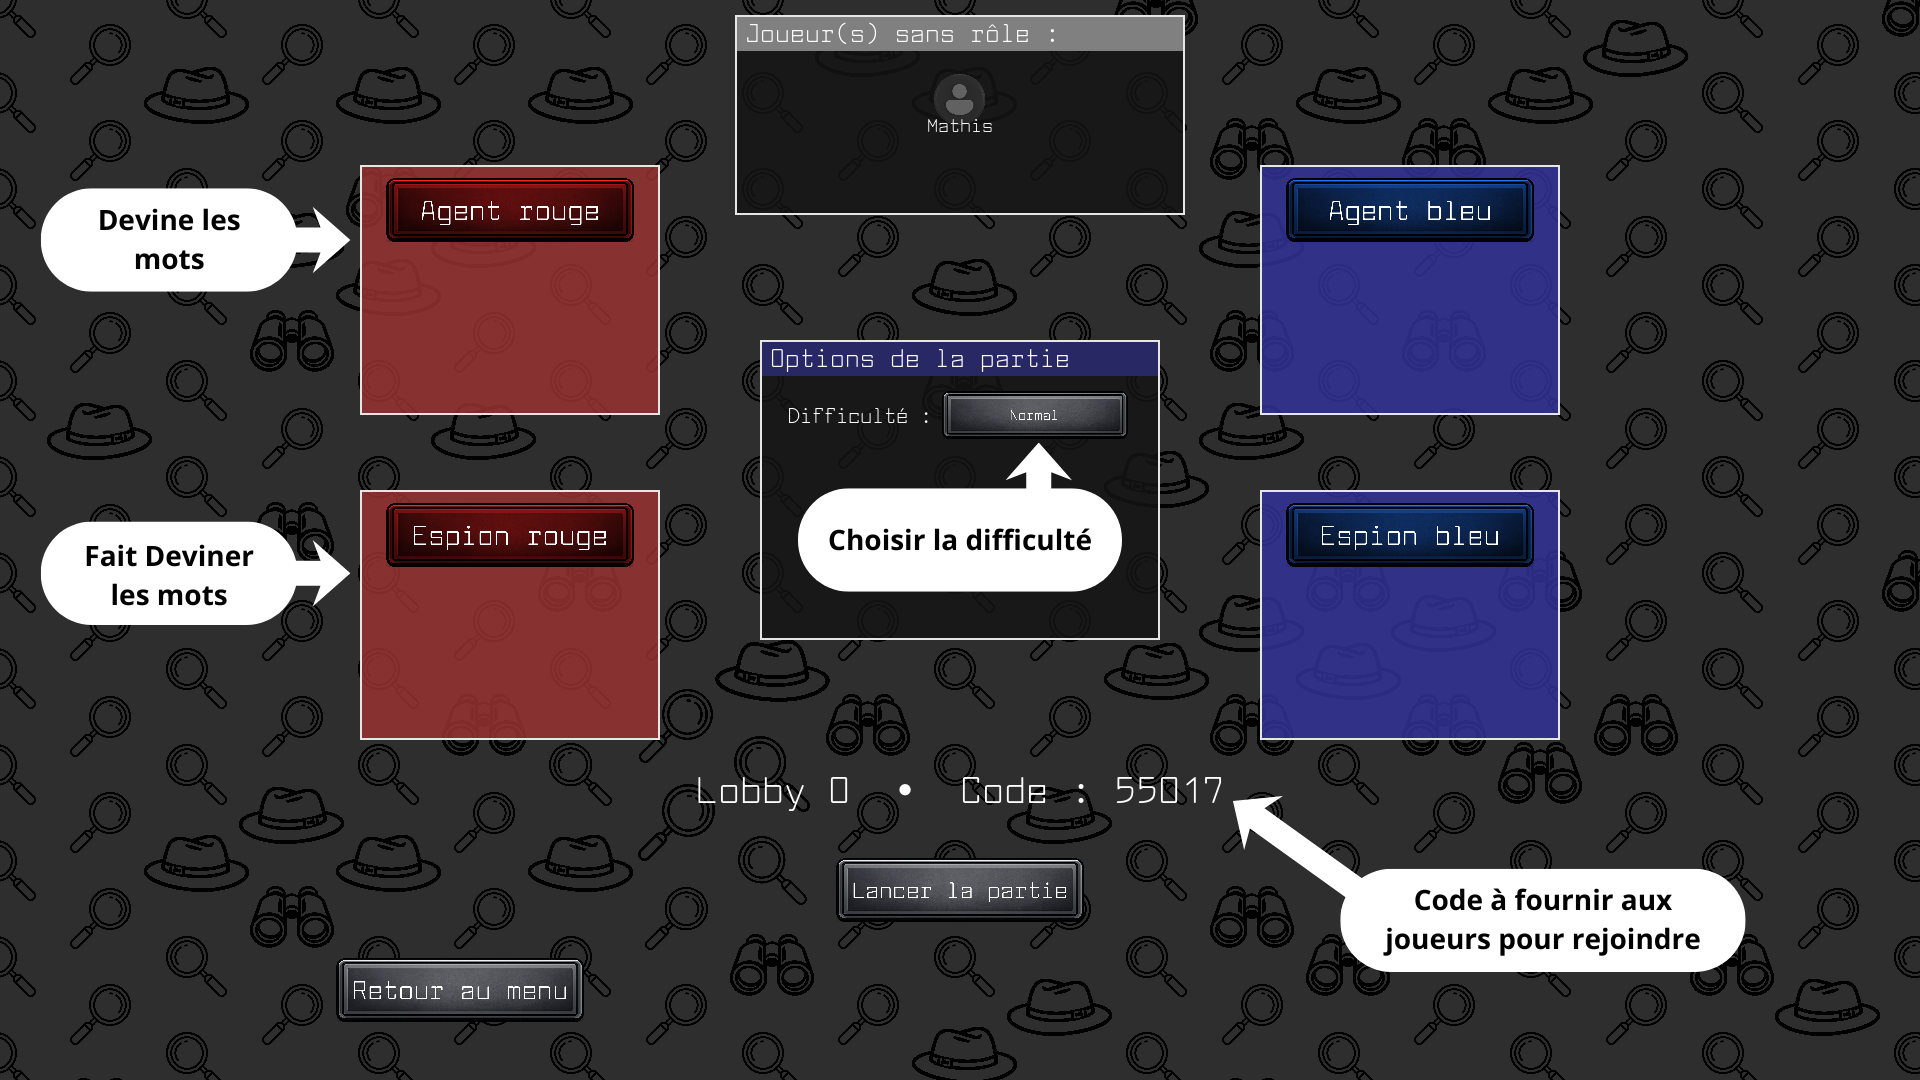
\includegraphics[width=\textwidth]{assets/annexes/tuto/tuto2.png}
        \caption{Page 2 du tutoriel}
        \label{fig:tuto2}
    \end{figure}
    \begin{figure}[H]
        \centering
        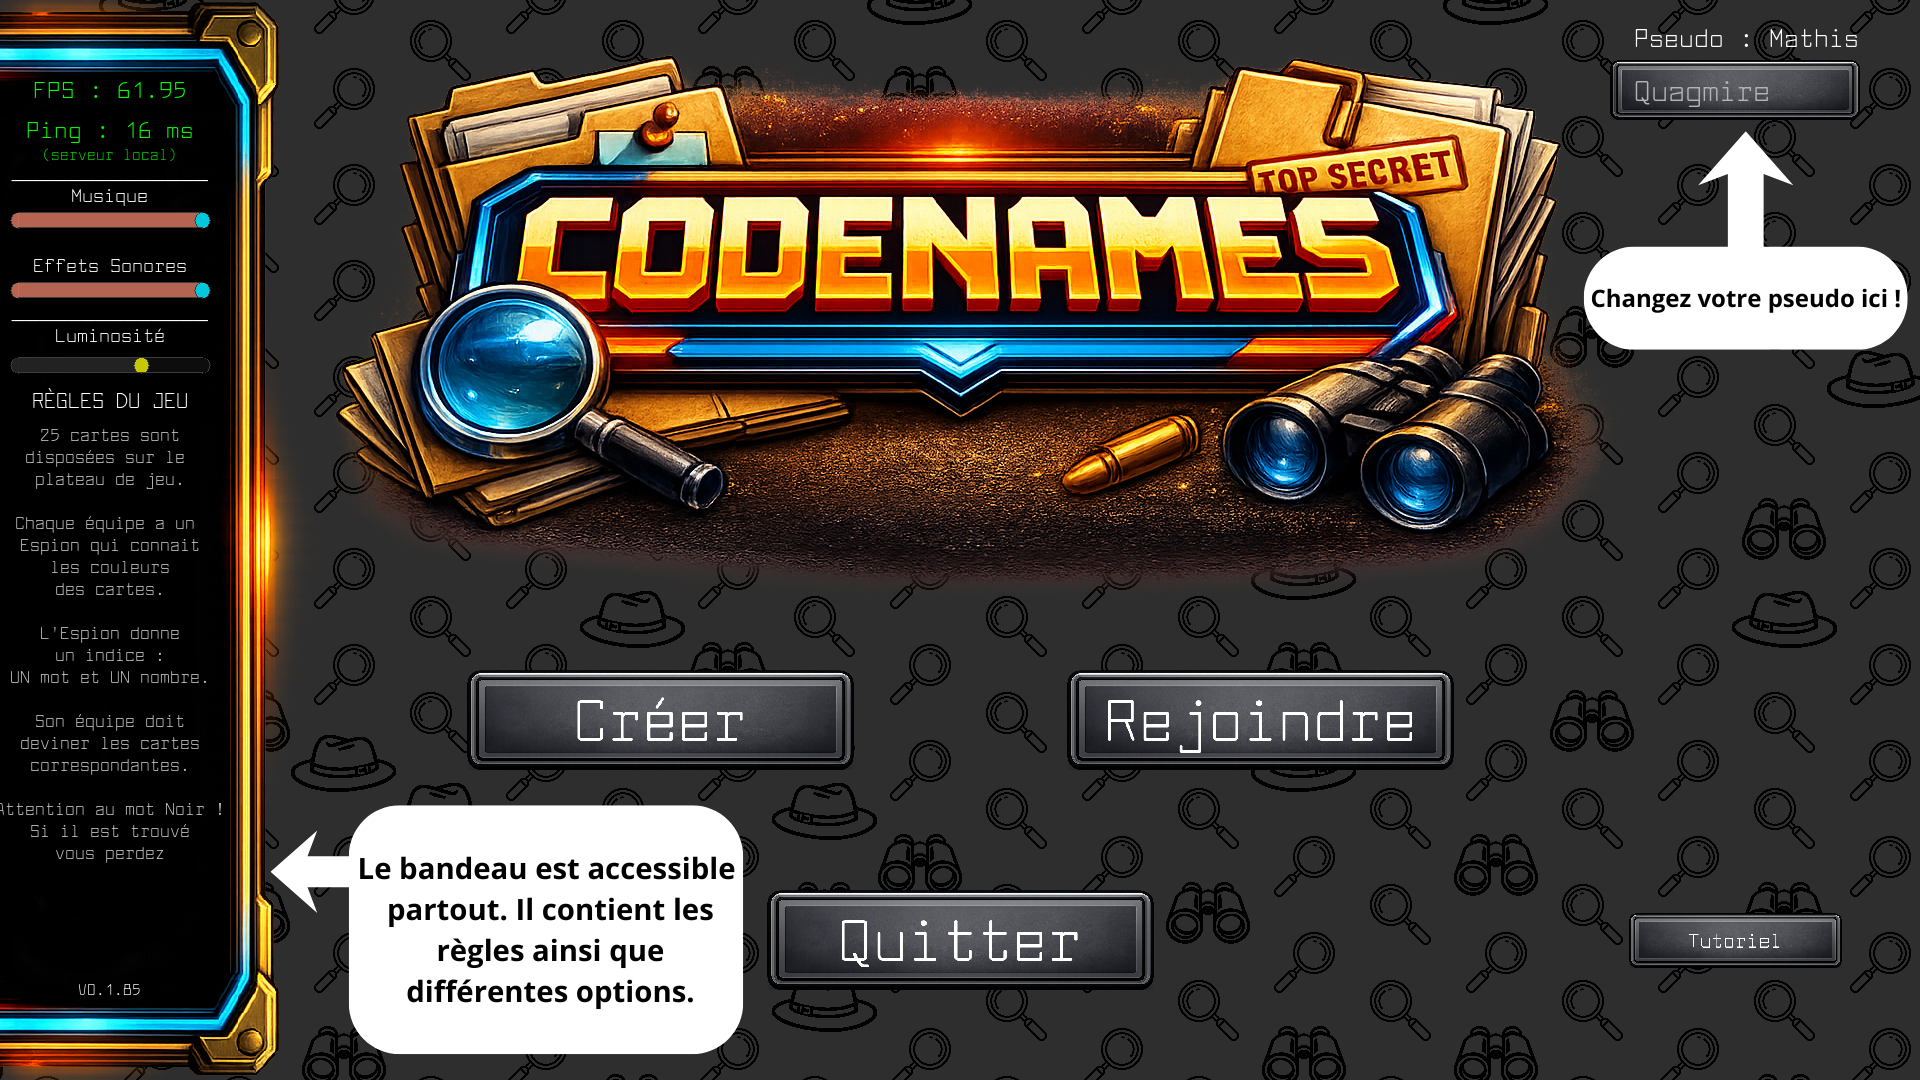
\includegraphics[width=\textwidth]{assets/annexes/tuto/tuto3.png}
        \caption{Page 3 du tutoriel}
        \label{fig:tuto3}
    \end{figure}
    \begin{figure}[H]
        \centering
        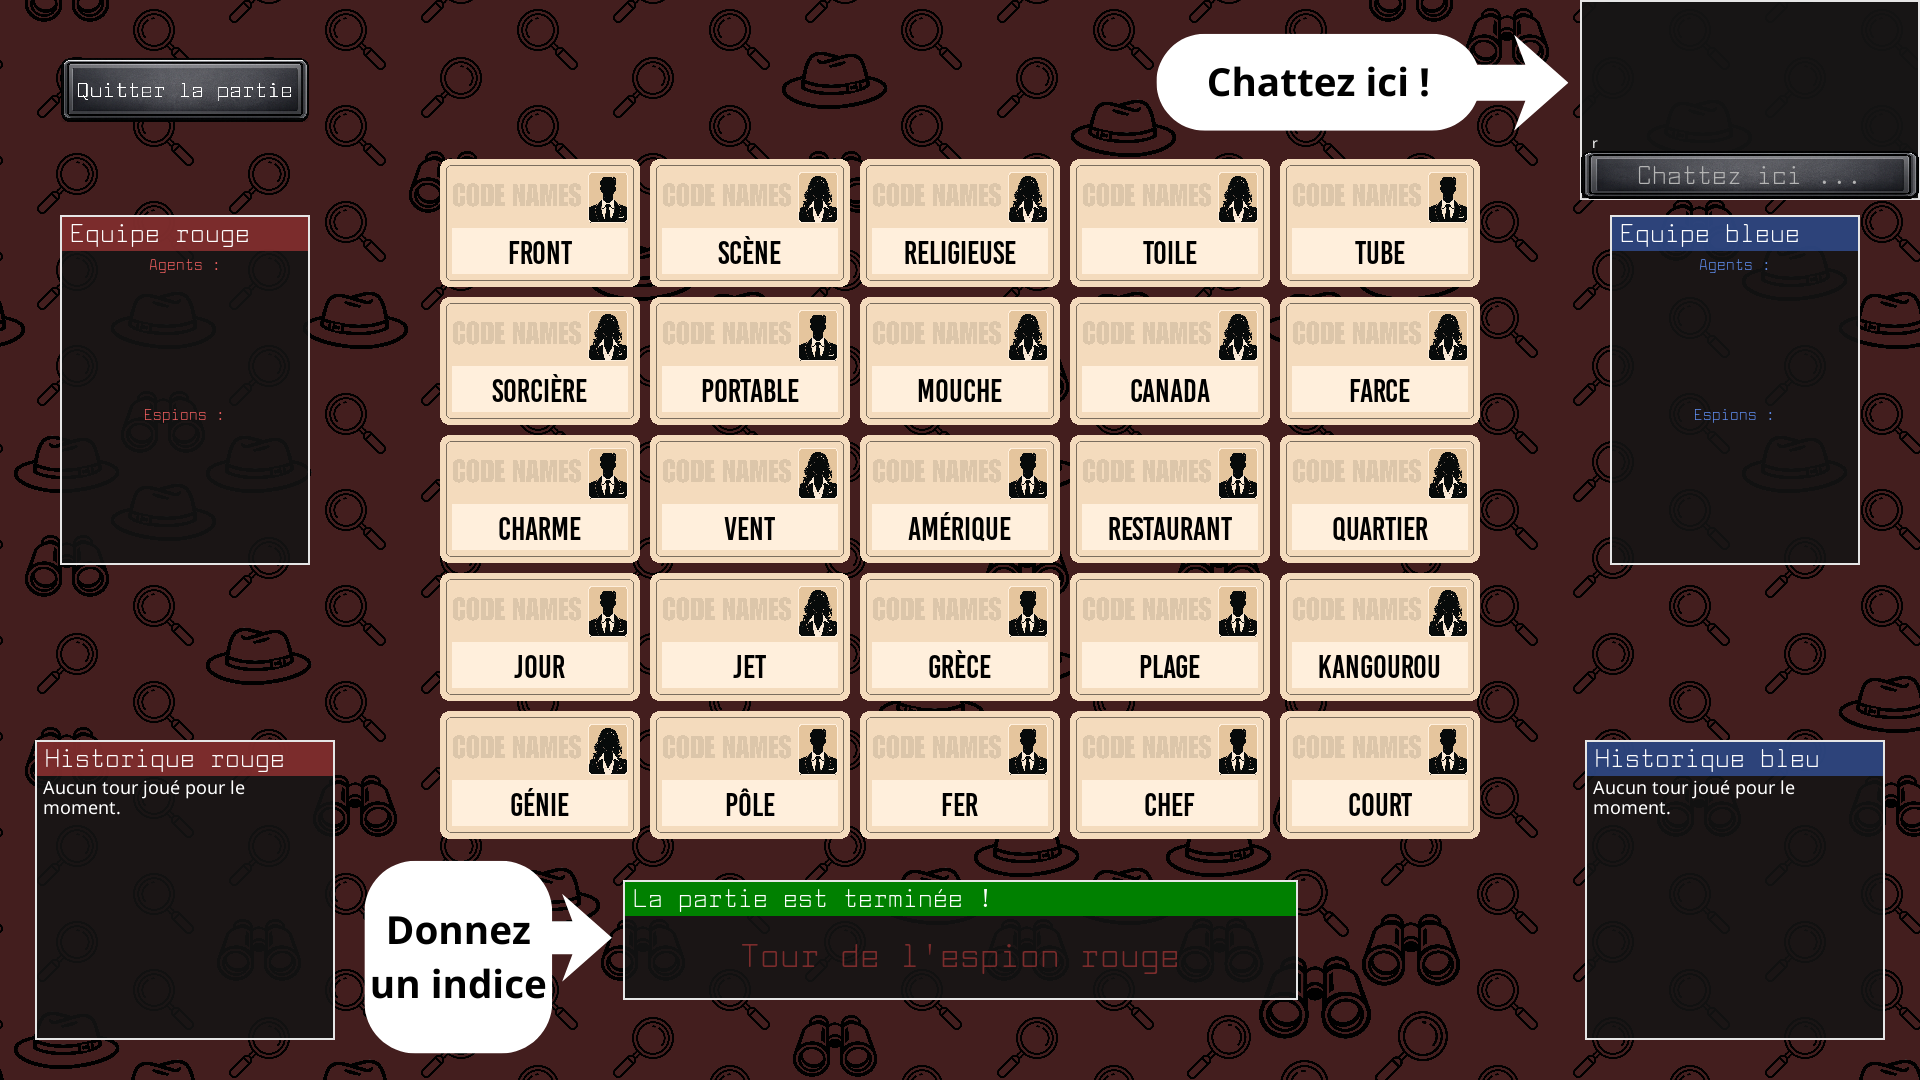
\includegraphics[width=\textwidth]{assets/annexes/tuto/tuto4.png}
        \caption{Page 4 du tutoriel}
        \label{fig:tuto4}
    \end{figure}

    \subsection{Exemple de partie}
    \begin{figure}[H]
        \centering
        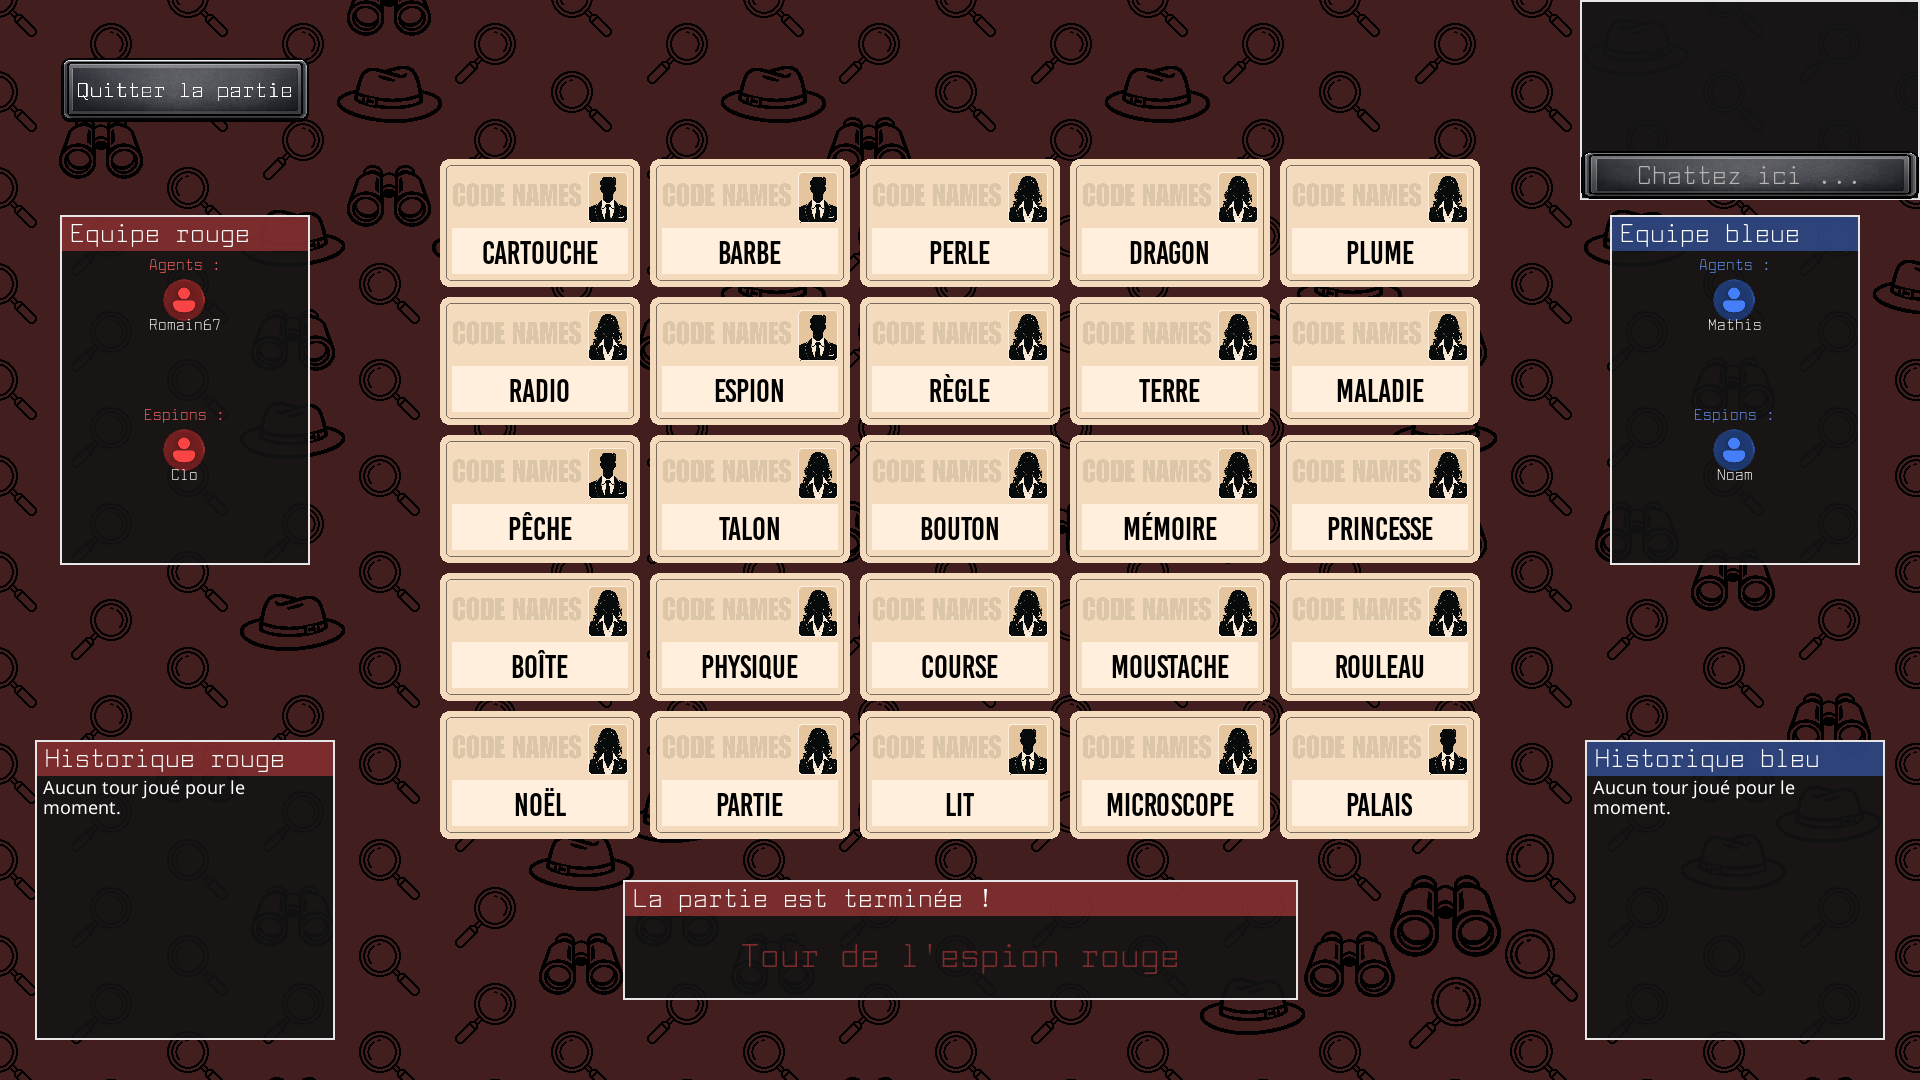
\includegraphics[width=\textwidth]{assets/annexes/partie/debut_agent.png}
        \caption{Début de partie pour un agent}
        \label{fig:debut_agent}
    \end{figure}
    \begin{figure}[H]
        \centering
        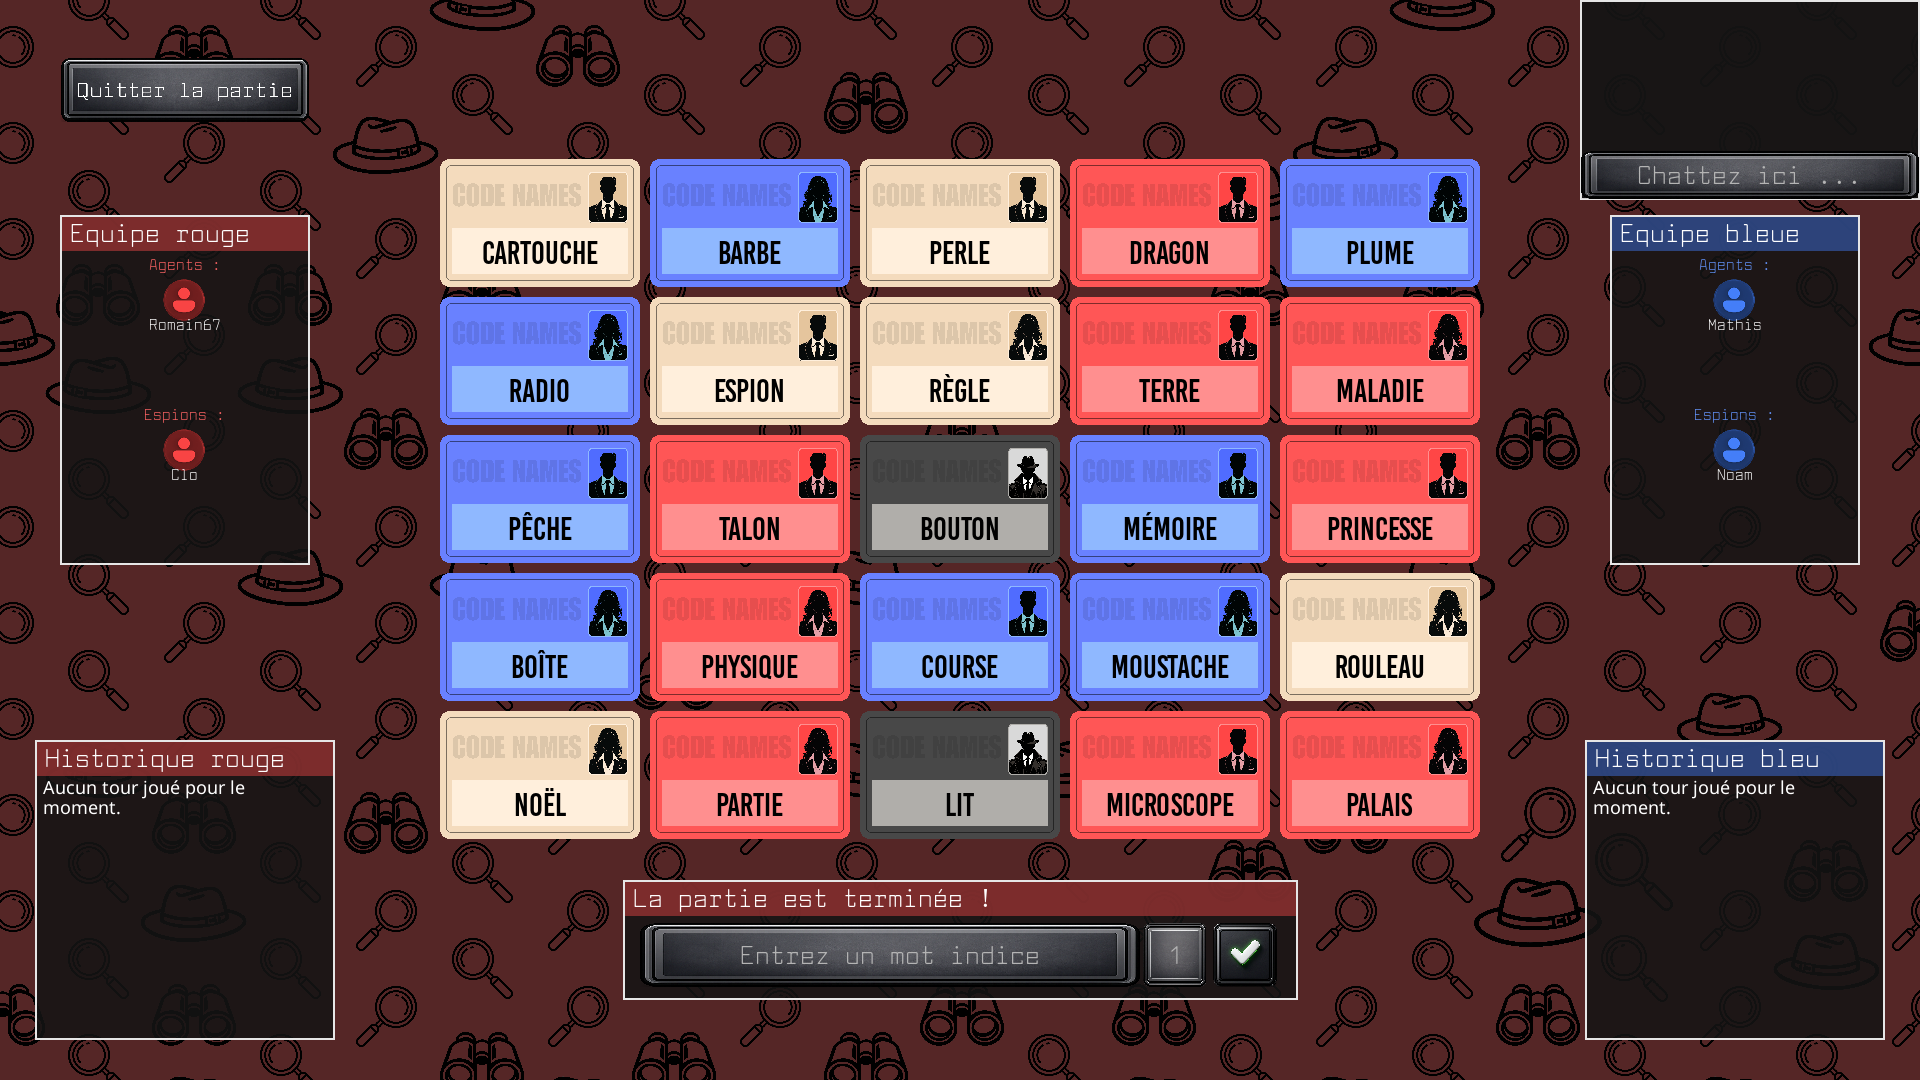
\includegraphics[width=\textwidth]{assets/annexes/partie/debut_espion.png}
        \caption{Début de partie pour un espion}
        \label{fig:debut_espion}
    \end{figure}
    \needspace{5\baselineskip}
    Le début de partie est différent selon le rôle du joueur, le point de vue d'un agent est montré dans la figure \ref{fig:debut_agent} et celui d'un espion dans la figure \ref{fig:debut_espion} ci-dessus.\\
    Dans cet exemple, on peut voir que 2 assasins ont été choisis pour cette partie, ce qui est une option disponible dans le lobby.
    Les rouges commencent, ils ont donc 9 mots à trouver contre 8 pour les bleus.

    \vspace{0.5cm}

    \begin{figure}[H]
        \centering
        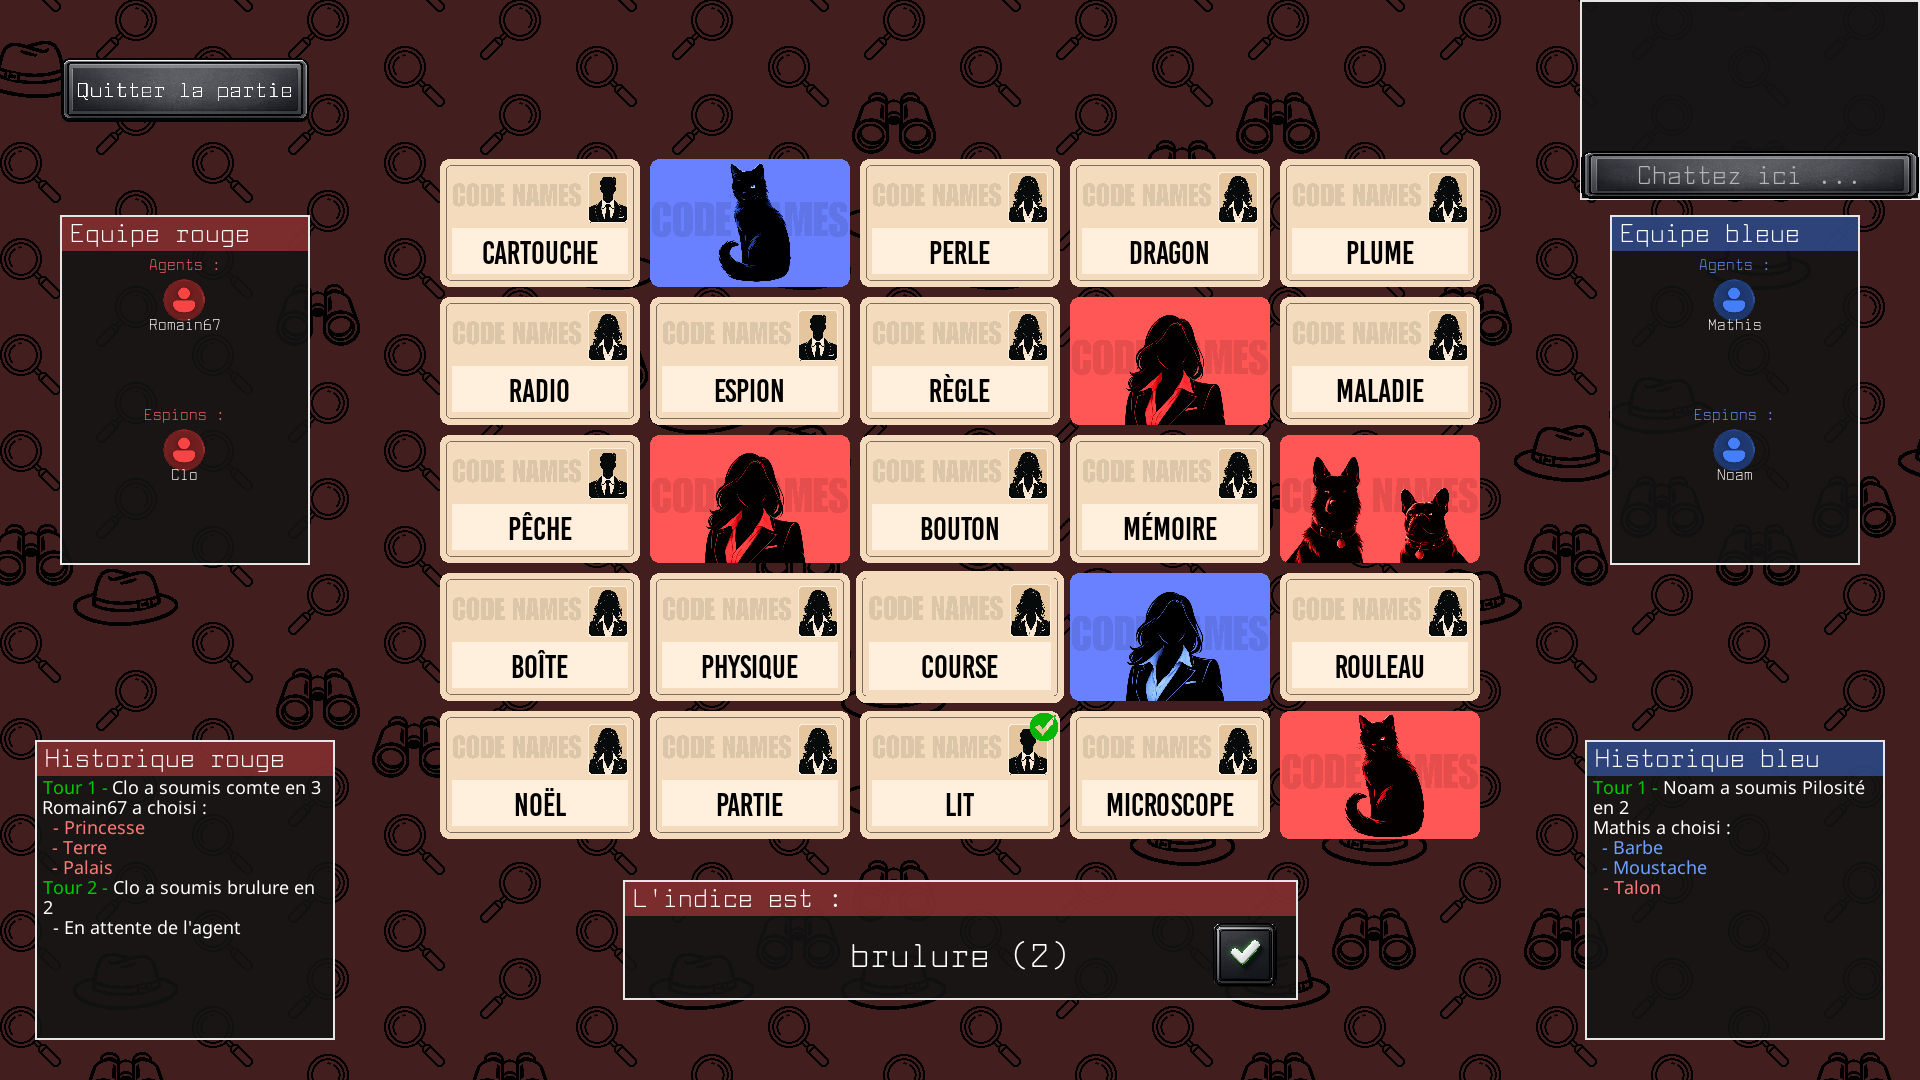
\includegraphics[width=\textwidth]{assets/annexes/partie/cours_de_partie_agent.png}
        \caption{Cours de partie pour un agent}
        \label{fig:cours_de_partie_agent}
    \end{figure}
    \begin{figure}[H]
        \centering
        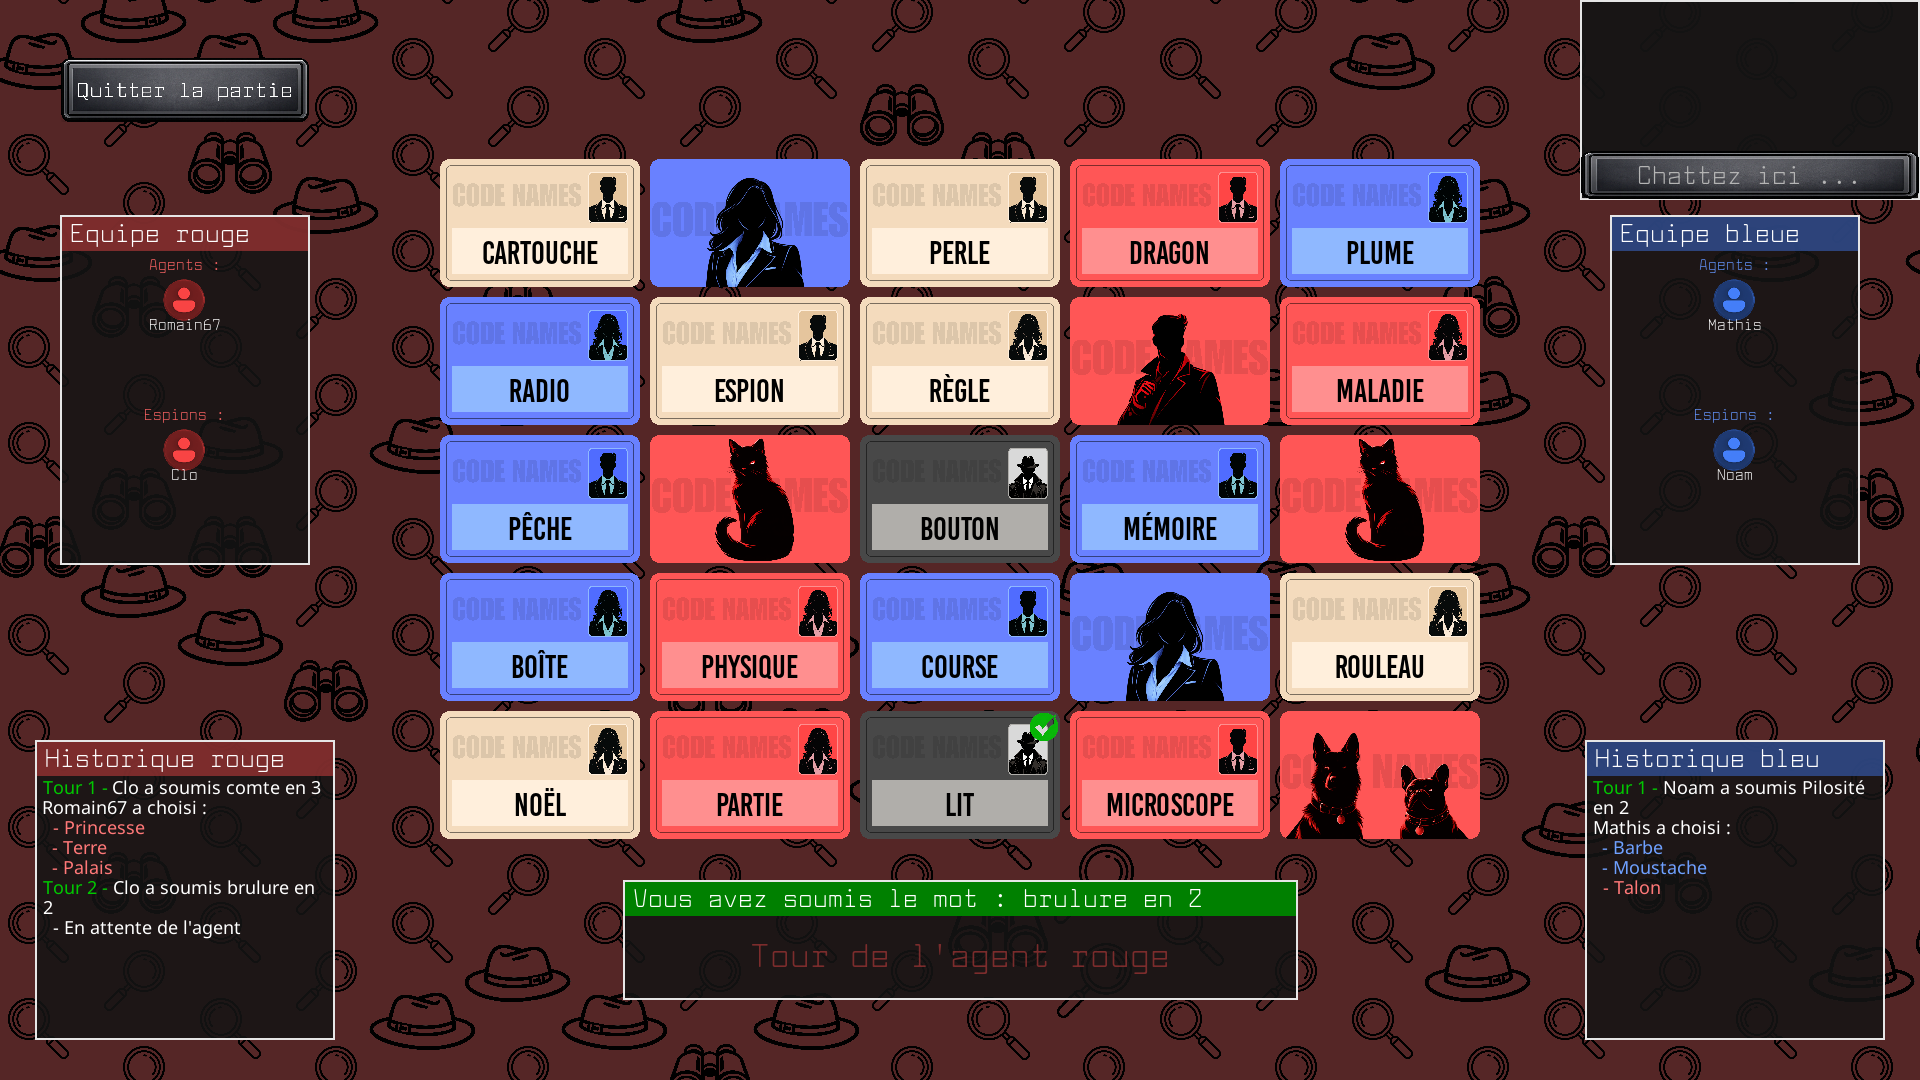
\includegraphics[width=\textwidth]{assets/annexes/partie/cours_de_partie_espion.png}
        \caption{Cours de partie pour un espion}
        \label{fig:cours_de_partie_espion}
    \end{figure}
    Le cours de partie est également différent selon le rôle du joueur, le point de vue d'un agent est montré dans la figure \ref{fig:cours_de_partie_agent} et celui d'un espion dans la figure \ref{fig:cours_de_partie_espion} ci-dessus.
    À ce moment de la partie, le fond est de couleur rouge pour indiquer que c'est au tour de l'équipe rouge de jouer. L'espion de l'équipe rouge a donné l'indice \og Brulure 2 \fg{}, son agent a préselectionné le mot \og lit \fg{}.
    Ici, 3 mots rouges ont été trouvés et 2 mots bleus ont été trouvés, on peut retrouver les indices et les mots trouvés dans les historiques en bas de l'écran.
    
    \vspace{0.5cm}
    
    \begin{figure}[H]
        \centering
        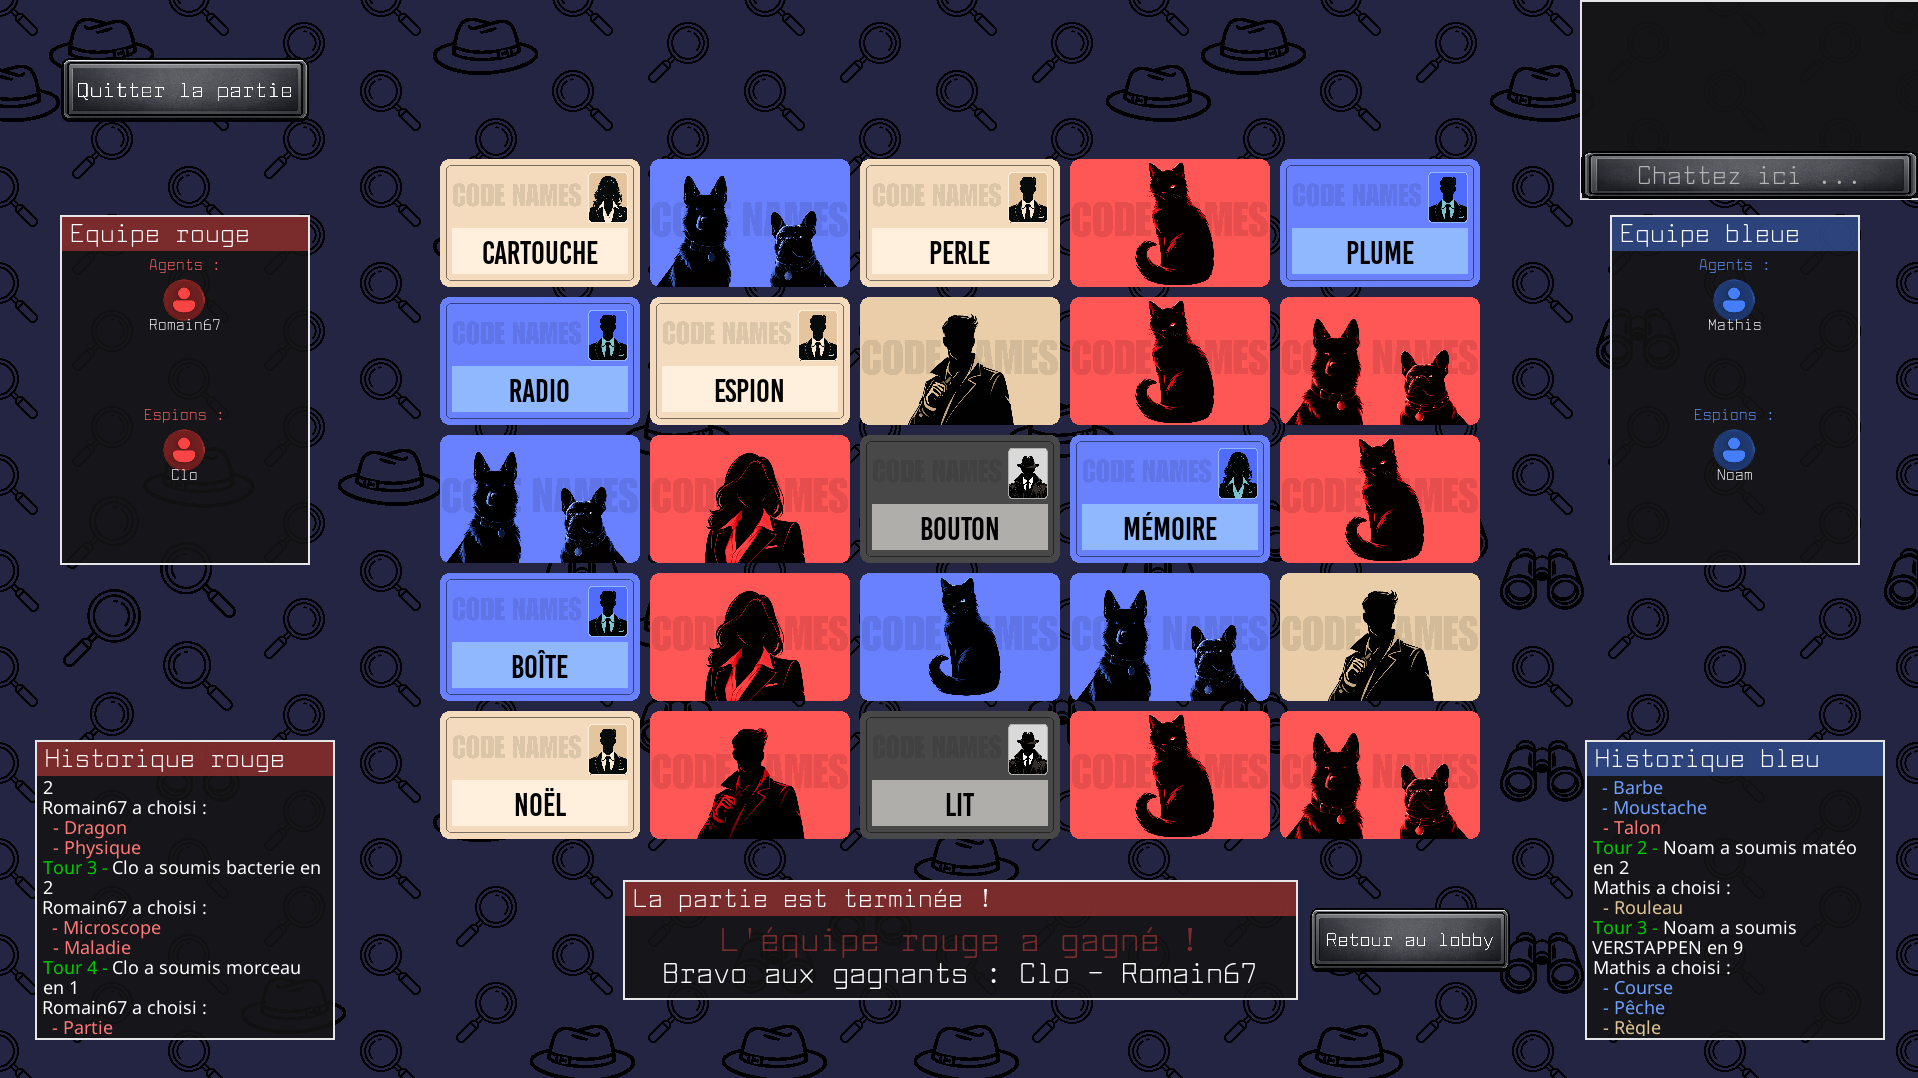
\includegraphics[width=\textwidth]{assets/annexes/partie/fin_de_partie.png}
        \caption{Fin de partie pour tous les joueurs}
        \label{fig:fin_de_partie}
    \end{figure}
    La fin de partie est la même pour tous les joueurs, comme montré dans la figure \ref{fig:fin_de_partie} ci-dessus.\\
    Elle affiche le résultat de la partie, ici les joueurs de l'équipe rouge ont gagné (\og \textcolor{red}{L'équipe rouge a gagné !} \fg, \og Bravo aux gagnants : Clo - Romain67 \fg).
    


\end{document}
